\documentclass{article}

\usepackage[utf8]{inputenc}
\usepackage{graphicx}
\usepackage{amsfonts}
\usepackage{amsmath}
\usepackage{indentfirst}
\usepackage{setspace}
\usepackage[procnames]{listings}
\usepackage{color}
\usepackage{multirow}

\setstretch{1.2}

\title{01. One Dimensional Motions}
\author{20191123\\Park Won}
\date{}

\begin{document}

\maketitle

\section{Purpose}


\section{Theoretical Background}


\section{Procedure}

\subsection{Linear Uniform Motion}


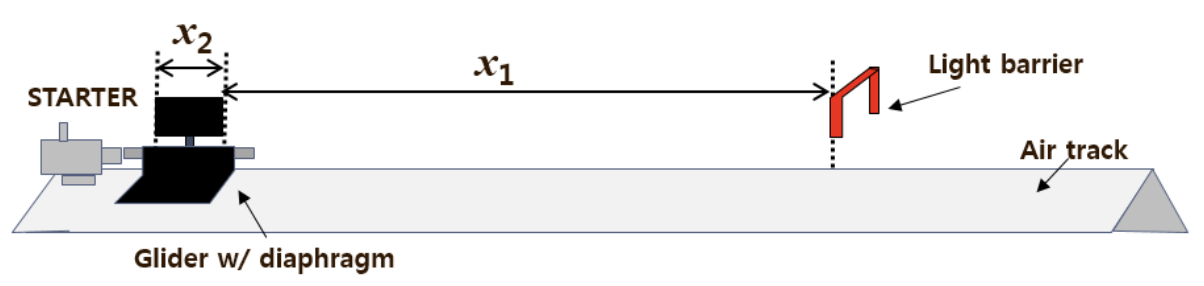
\includegraphics[width=\columnwidth]{A.png}


\subsection{Uniformly Accelerated Motion with on Inclined Track}


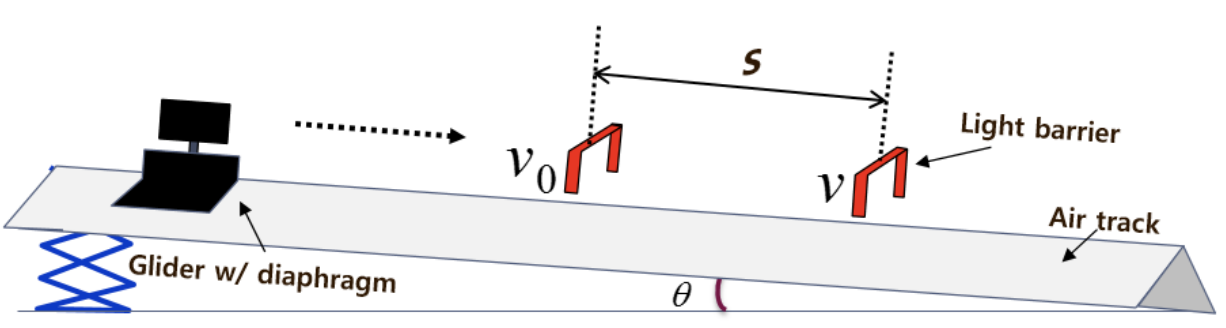
\includegraphics[width=\columnwidth]{B.png}


\subsection{Uniformly Accelerated Motion with on Accelerating Mass}


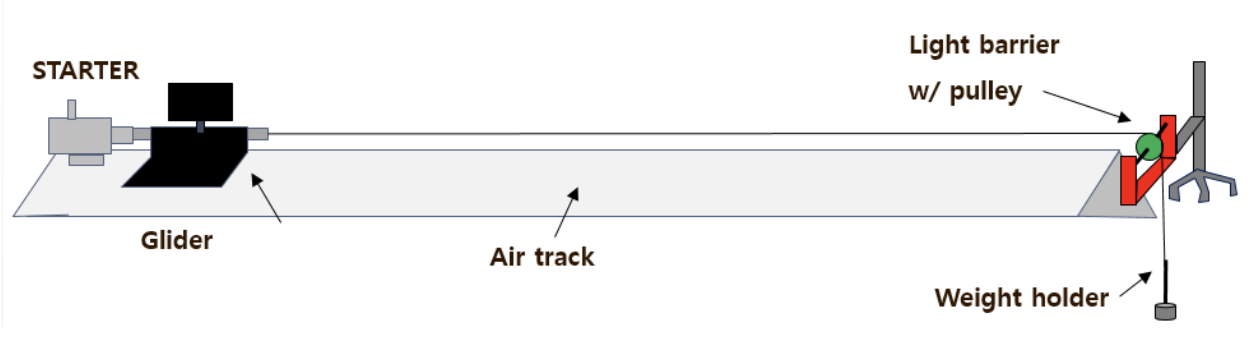
\includegraphics[width=\columnwidth]{C.png}


\section{Data Analisys and Conclusion}

\subsection{Linear Uniform Motion}

\begin{table}[h!]
\centering
\begin{tabular}{}
\end{tabular}
\caption{mass of the glider and parts}
\label{table:1}
\end{table}

\begin{table}[h!]
\centering
\begin{tabular}{}
\end{tabular}	
\caption{The velocity measured from timer 1($v_1$) and timer 2($v_2$)}
\label{table:2}
\end{table}

\begin{table}[h!]
\centering
\begin{tabular}{}
\end{tabular}
\caption{The velocity of the glider which is slotted weight (with 0.8m)}
\label{table:3}
\end{table}

\subsection{Uniformly Accelerated Motion with an Inclined Track}


\begin{table}[h!]
\centering
\begin{tabular}{}	
\end{tabular}
\caption{The velocities of the accelerated glider on the inclined track}
\label{table:4}
\end{table}


\subsection{Uniformly Accelerated Motion with an Accelerating Mass}

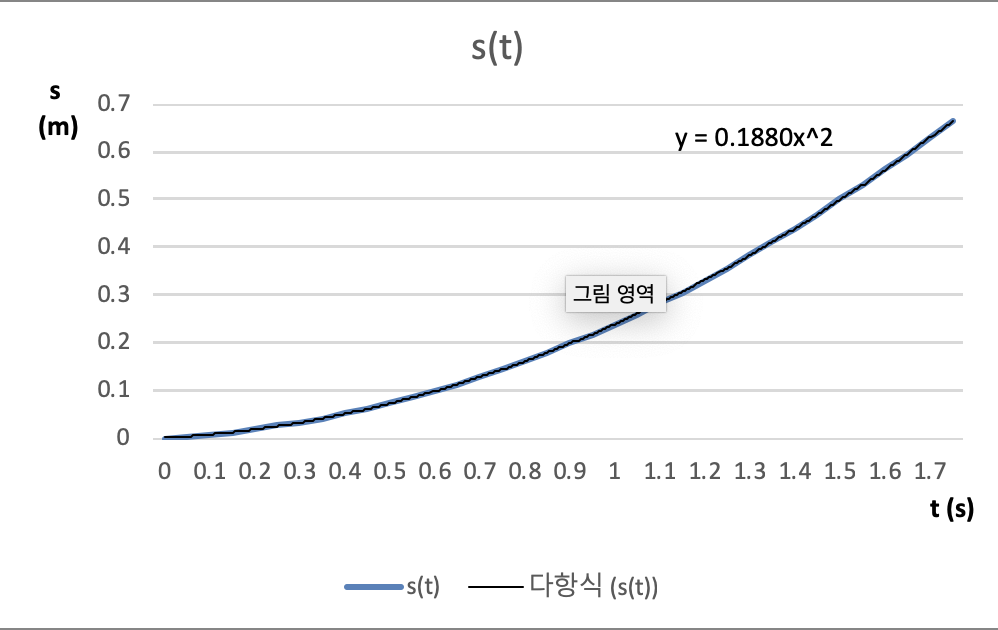
\includegraphics[width=\columnwidth]{S.png}

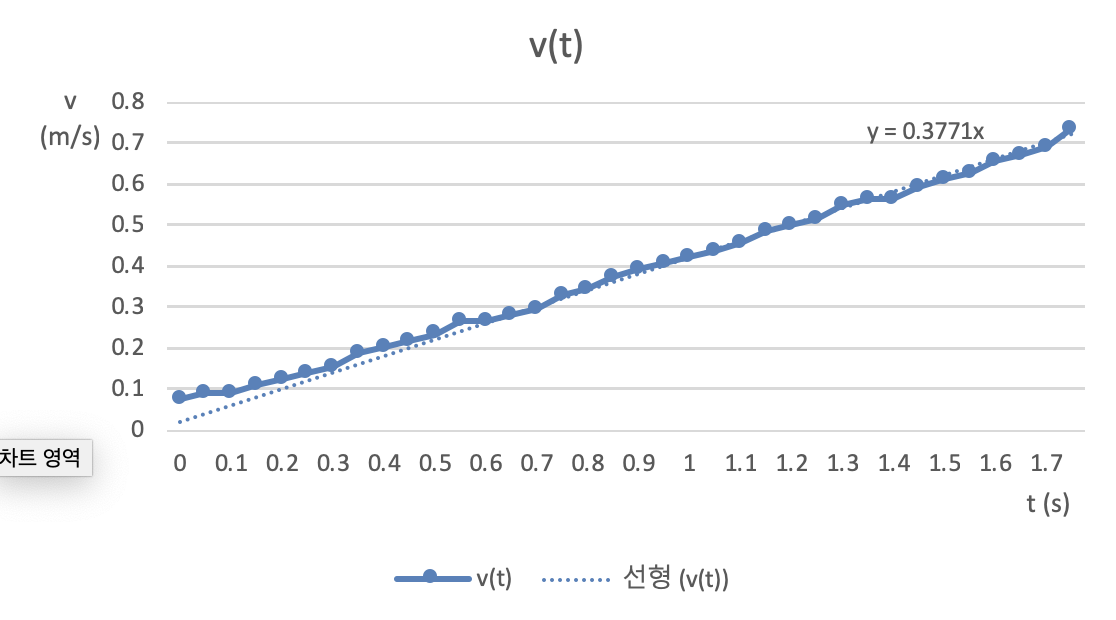
\includegraphics[width=\columnwidth]{V.png}

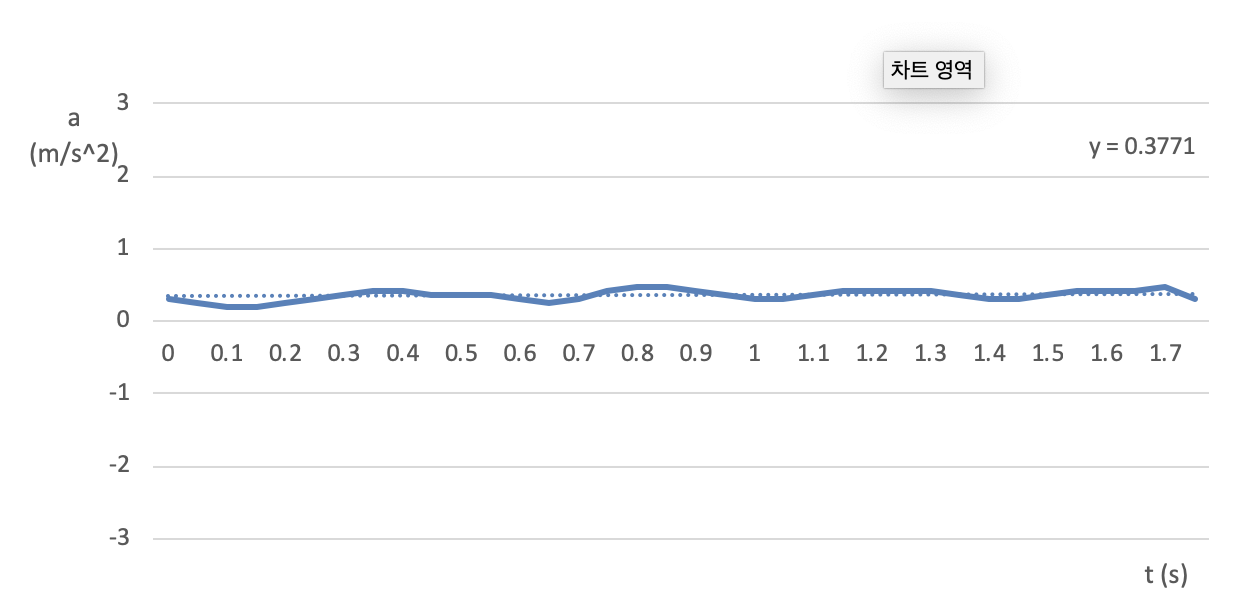
\includegraphics[width=\columnwidth]{AC.png}

\end{document}